\chapter{Materials \& Methods}

%\textbf{This section should include a recipe of what you did (explain what you have done so if someone wants to reproduce the experiment, they can).  A flow chart is typically helpful.  Also, make sure to define all software that you used including version numbers and OS.  Should also include a description of statistical methods used (if any).\footnote{For more information see: \url{http://rc.rcjournal.com/content/49/10/1229.short}}}

For this \ac{IAPT} a multi-stage approach was used for data collection, analyses and evaluation.
This approach is described in figure~\ref{fig:flowchart} as a flowchart.

\begin{figure}[h!]
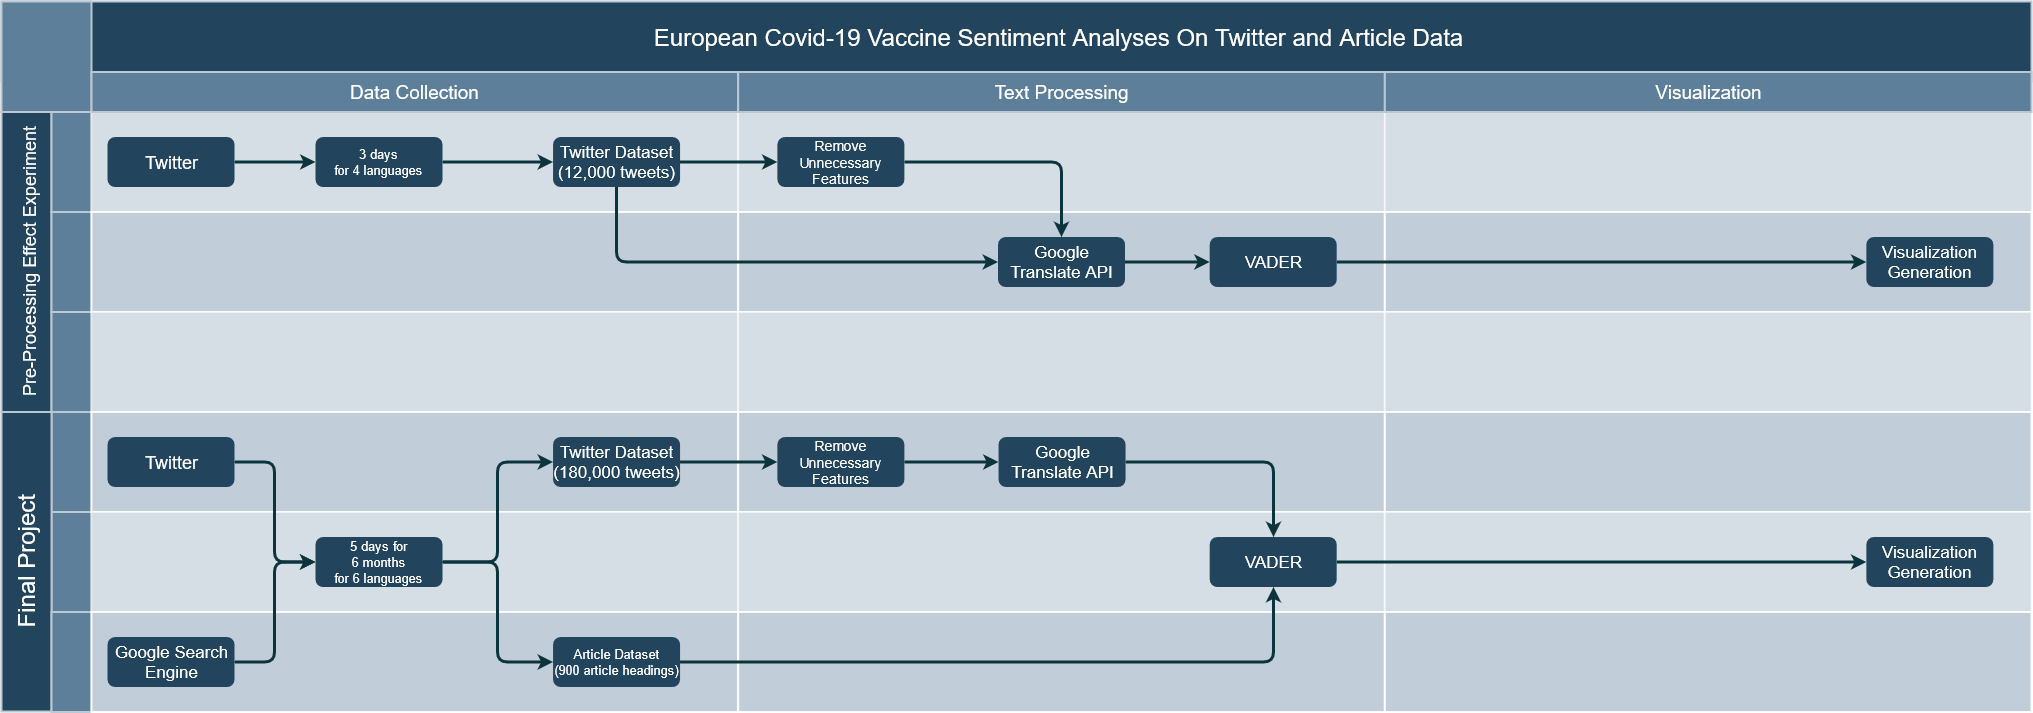
\includegraphics[scale=0.2]{IAPT Flowchart}
\caption[Method Flowchart]{Flowchart of the Method of Experiment\index{Method Flowchart}}
\label{fig:flowchart}
\end{figure}

\section{Data Collection}
asd
\subsection{Twitter Dataset}
asd
\subsection{Article Dataset}
asd

\section{Data Processing}
asd

\section{Sentiment Analyses}
asd

\section{Visualization}
asd
\Blindtext

\section{Summary}
\blindtext